\documentclass[../differential_topology.tex]{subfiles}
\begin{document}
\section{Aula 07 - 15 de Setembro, 2026}
\subsection{Motivações}
\begin{itemize}
	\item Estabilidade
\end{itemize}
\subsection{Estabilidade}
\begin{def*}
	Duas aplicações \(f_{0},\; f:M\rightarrow N\) suaves são \textbf{homotópicas} se existe aplicação suave \(F:M\times I\rightarrow N\), onde I é o intervalo \(I=[0,1]\), tal que:
	\begin{itemize}
		\item[1)] \(F(x, 0) = f_{0}\);
		\item[2)] \(F(x, 1) = f.\)
	\end{itemize}
	Caso exista uma aplicação assim, diremos que F é uma \textbf{homotopia entre \(\mathbf{f_{0}}\) e \(\mathbf{f}\)}. \(\square\)
\end{def*}
Isso define uma classe de funções dadas por \(F_{t}:M\rightarrow N,\; F_{t}(x) = F(x, t)\), onde t é um valor entre 0 e 1; mais ainda, uma homotopia é uma relação de equivalência, significando que podemos usar as classes de equivalência, chamadas \textbf{classes de homotopia}, como uma partição do espaço \(\mathcal{C}^{\infty}(M, N)\).
Em termos escritos, duas aplicações são homotópicas se elas podem ser ligadas por um caminho:
\begin{figure}[H]
	\begin{center}
		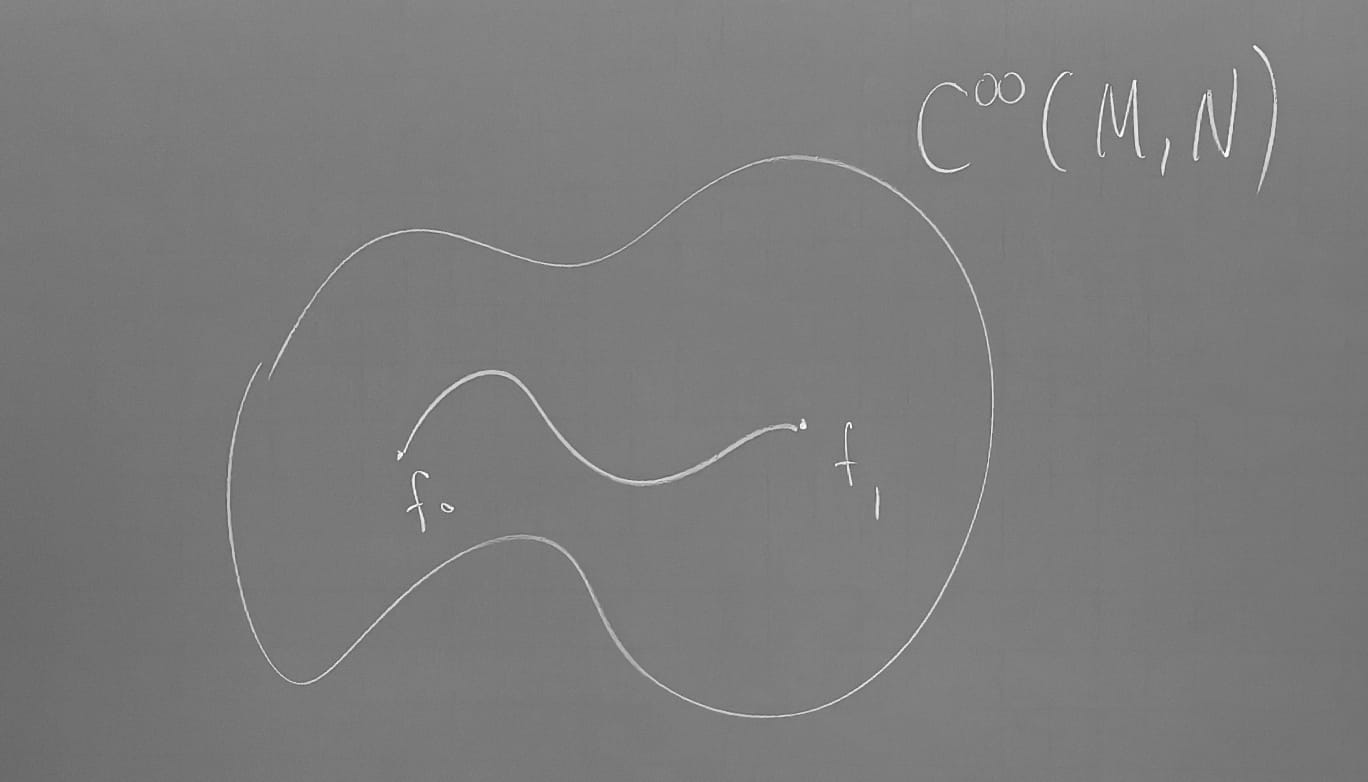
\includegraphics[height=\textheight, width=\textwidth, keepaspectratio]{./Images/07_homotopy.png}
	\end{center}
\end{figure}

\begin{def*}
	Uma aplicação \(f_{0}:M\rightarrow N\) suave possuir uma propriedade ``P'' \textbf{estável} se existe \(F:M\times I\rightarrow N\) suave tal que:
	\begin{itemize}
		\item[1)] \(F_{0} = f_{0}\); e
		\item[2)] Existe \(\varepsilon >0\) tal que \(F_{t}\) possui a propriedade ``P'' para todo t em \([0, \varepsilon ).\; \square\)
	\end{itemize}
\end{def*}
Poderíamos pensar nesse tipo de estabilidade em específico como \textit{estabilidade por caminhos}, pois a definição é que existe um caminho no qual todos os pontos de um certo segmento dele possuem a mesma propriedade que a aplicação \(f\).
Pela teoria desenvolvida até aqui, temos uma família de aplicações que são estáveis nesse sentido!

\begin{theorem*}
	As seguintes classes de aplicações suaves entre variedades compactas são estáveis:
	\begin{itemize}
		\item[i)] Difeomorfismos locais;
		\item[ii)] Imersões;
		\item[iii)] Submersões;
		\item[iv)] Aplicações transversais a uma subvariedade \textit{fixa};
		\item[v)] Mergulhos; e
		\item[vi)] Difeomorfismos.
	\end{itemize}
\end{theorem*}
Os itens (i)-(iii) podem ser resumidos como ``aplicações com \hyperlink{max_rank}{\textit{posto máximo}} são estáveis'' (ou melhor, a derivada em um ponto p tem ponto máximo)
Em todos eles, a ideia do argumento seria que, com respeito ao jacobiano, modificações pequenas em torno de uma vizinhança dele, que é uma função contínua, ainda são provavelmente não nulas, preservando a propriedade que requer que o determinante seja não nulo.
A da transversalidade, por sua vez, se baseia no princípio de que bastaria uma pequena modificação na linha com o caminho perturbado para recuperar a linha transversal quando olha-se pro espaço tangente escalado pela função perturbada.
\begin{figure}[H]
	\begin{center}
		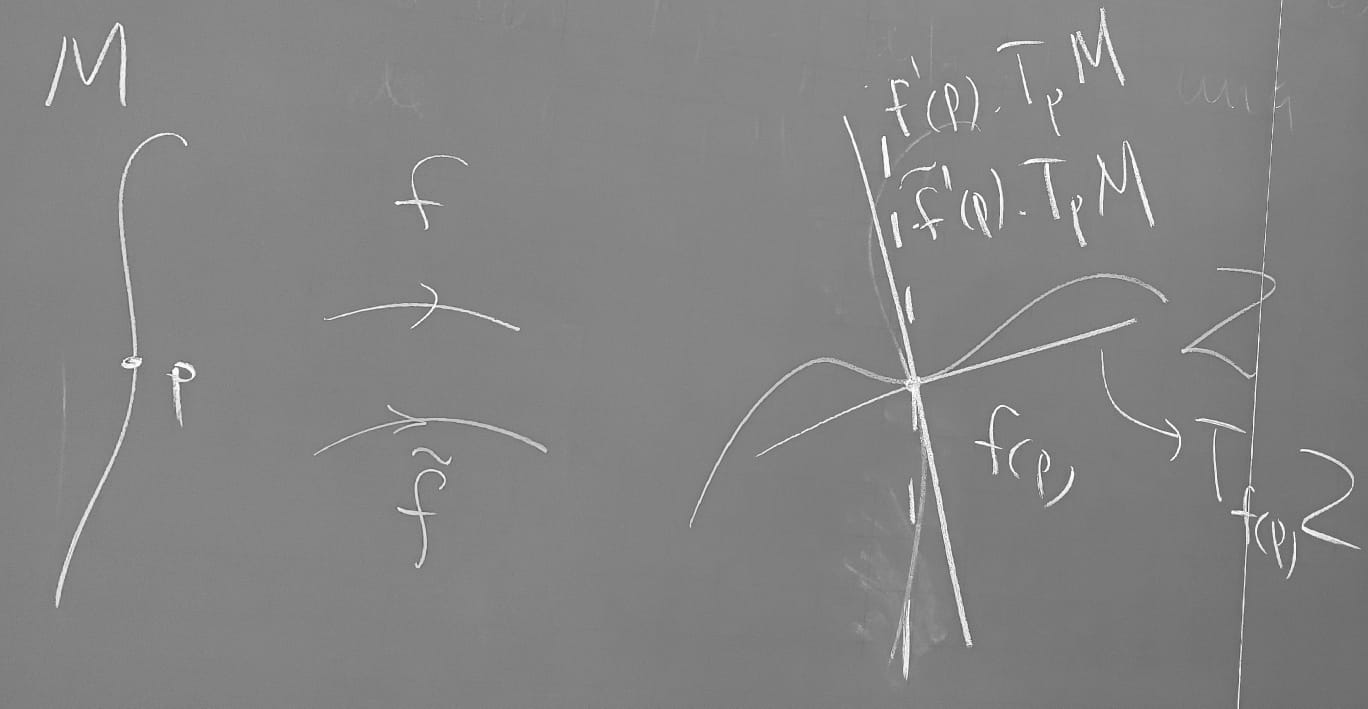
\includegraphics[height=\textheight, width=\textwidth, keepaspectratio]{./Images/07_stability.png}
	\end{center}
\end{figure}

\begin{tcolorbox}[
		skin=enhanced,
		title=Lembrete!,
		after title={\hfill Posto Máximo},
		fonttitle=\bfseries,
		sharp corners=downhill,
		colframe=black,
		colbacktitle=yellow!75!white,
		colback=yellow!30,
		colbacklower=black,
		coltitle=black,
		%drop fuzzy shadow,
		drop large lifted shadow
	]
	Uma aplicação suave tem \hypertarget{max_rank}{\textbf{Posto Máximo}} se a matriz Jacobiana de f tem posto dado pelo mínimo entre as dimensões das variedades; por exemplo, se \(f:M\rightarrow N,\; \mathrm{dim}(M) = m,\; \mathrm{dim}_{}(N)=n\), então f será de posto máximo se \(\mathrm{rank}(\mathrm{d}f_{p})=\min\limits_{}\{m, n\}\), e pode parecer estranho o nome ser ``posto máximo'' usando um mínimo para definí-lo, mas é porque
	\[
		\mathrm{rank}(\mathrm{d}f_{p})\leq \min\limits_{}\{m, n\},
	\]
	ou seja, a igualdade é o valor máximo.

	Quando m for o mínimo, segue que \(\mathrm{rank}(\mathrm{d}f_{p})=m\), ou seja, \(\mathrm{d}f_{p}\) é injetiva, e f é uma imersão! Analogamente, o outro caso resulta em \(\mathrm{d}f_{p}\) sendo sobrejetora, levando a f ser uma submersão.
	Em particular, se \(m=n\), o posto máximo significa que \(\mathrm{d}f_{p}\) é um isomorfismo, tal que a função f será um difeomorfismo local.
\end{tcolorbox}

\subsection{Teorema de Sard}
\begin{def*}
	Seja \(f:M\rightarrow N\) uma aplicação suave; diremos que um ponto \(p\in M\) é um \textbf{ponto crítico} se \(f'(p)\) não tem um ponto máximo, caso no qual diremos que \(f(p)\) é um \textbf{valor crítico}.
	Diremos que \(p\) é \textbf{ponto regular} se p não é um ponto crítico, e que \(f(p)\) é um \textbf{valor regular} se \(p\) for um ponto regular. \(\square\)
\end{def*}
Um ponto crítico ocorre quando a derivada não é difeomorfismo local, nem isomorfismo, nem sobrejetora, nem injetora.
\begin{def*}
	Um \textbf{conjunto de medida nula em espaços euclidianos} é um subconjunto \(A\subseteq \mathbb{R}^{\ell }\) tal que, para cada \(\varepsilon > 0\), existe uma família enumerável de retângulos \(\{R_{i}\}_{i\in \mathbb{N}}\) em \(\mathbb{R}^{\ell }\) tais que
	\[
		\left\{\begin{array}{ll}
			\bigcup_{i}^{}R_{i} \supseteq A \\
			\sum\limits_{i}^{}\mathrm{vol}(R_{i}) < \varepsilon
		\end{array}\right.
	\]
	O volume é o produto dos lados, como esperado pro produto de intervalos. \(\square\)
\end{def*}
\begin{def*}
	Seja M uma variedade suave; um subconjunto \(C\subseteq M\) tem \textbf{medida nula} se, para cada parametrização \(\varphi :U\subseteq \mathbb{R}^{m}\rightarrow V\subseteq M\), a pré-imagem \(\varphi^{-1}(C\subseteq V)\subseteq \mathbb{R}^{m}\) tem medida nula. \(\square\)
\end{def*}
O gráfico de funções tem medida nula, garantindo que qualquer subvariedade própria tenha medida nula, pois são localmente definidas em termos de aplicações, logo têm medida nula também!

\hypertarget{sard_theorem}{
	\begin{theorem*}[Teorema de Sard-Morse]
		O conjunto dos valores críticos de uma aplicação suave \(f:M\rightarrow N\) tem medida nula (em N).
		Na verdade, a classe de diferenciabilidade da f necessária não é \(\infty\), mas pelo menos satisfazer \(f\in \mathcal{C}^{r}(M, N)\) com
		\[
			r\geq \max\limits\{m-n+1, 1\}
		\]
	\end{theorem*}
}

\begin{tcolorbox}[
		skin=enhanced,
		title=Observação,
		fonttitle=\bfseries,
		colframe=black,
		colbacktitle=cyan!75!white,
		colback=cyan!15,
		colbacklower=black,
		coltitle=black,
		drop fuzzy shadow,
		%drop large lifted shadow
	]
	O conjunto de valores regulares de \(f:M\rightarrow N\) é denso, fornecendo pontos onde a imagem inversa é uma subvariedade, além de que, numa vizinhança de um valor regular, todos os outros pontos também são! Podemos usar isso para construir decomposições em subvariedades, tipo um livro, mas as folhas não são retangulares e podem ter genus infinito...
	Se tivermos uma quantidade enumerável de aplicações suaves \(f_{i}:M\rightarrow N\), a interseção dos valores regulares de \(f_{i}\) será densa também, simplesmente porque a união enumerável de conjuntos de medida nula também tem medida nula.
\end{tcolorbox}

Restringindo às aplicações \(f:M\rightarrow \mathbb{R}\), vale que, se p é um ponto regular, então \(f'(p):T_{p}M\rightarrow \mathbb{R}\) é sobrejetora, tornando-a localmente equivalente à projeção canônica \(\pi :\mathbb{R}^{m-1}\times \mathbb{R}\rightarrow \mathbb{R}\)
Caso p não seja regular, não podemos transformar f em uma projeção; que tipos de pontos críticos podemos ter? Temos que nos basear na definição de um ponto crítico não degenerado:
\begin{def*}
	Um ponto \(p\in \mathbb{R}^{m}\) é um \textbf{ponto crítico não degenerado} de \(f:\mathbb{R}^{m}\rightarrow \mathbb{R}\) se a hessiana de \(f(p)\), matriz que reúne suas derivadas segundas, é não singular:
	\[
		\det{\mathrm{Hess}(f(p))} \neq 0, \quad \mathrm{Hess}(f(p)) = \begin{bmatrix}
			\frac{\partial^{2}f}{\partial x_1^{2}}              & \dotsc & \frac{\partial^{2}f}{\partial x_1 \partial x_{m}^{}} \\
			\vdots                                              & \ddots & \vdots                                               \\
			\frac{\partial^{2}f}{\partial x_{m}\partial x_1^{}} & \dotsc & \frac{\partial^{2}f}{\partial x_{m}^{2}}
		\end{bmatrix}.\; \square
	\]
\end{def*}
Logo, um ponto crítico de \(f\) é não degenerado quando a Hessiana de \(f\) aplicada a ele é invertível. No contexto de variedades,
\begin{def*}
	Um ponto p da variedade M é um \textbf{ponto crítico não degenerado} de \(f:M\rightarrow \mathbb{R}\) se, para cada parametrização \(\varphi :U\subseteq \mathbb{R}^{m}\rightarrow V\) de M em p com \(\varphi (0) =p,\) 0 é um ponto crítico não degenerado de \(f\circ \varphi.\; \square\)
\end{def*}
\begin{example}
	Consideremos a aplicação \(f:\mathbb{R}^{m}\rightarrow \mathbb{R}\) dada por
	\[
		f(x_1, \dotsc , x_{m}) = x_{1}^{2} +\dotsc +x_{p}^{2} - x_{p-1}^{2} -\dotsc -x_{m}^{2};
	\]
	como
	\[
		f'(0) = 0,
	\]
	vemos que 0 é um ponto crítico, e que a matriz Hessiana de f no ponto 0 é
	\[
		\mathrm{Hess}(f(0)) = \begin{bmatrix}
			2      & 0      & 0      & 0      & \dotsc \\
			0      & 2      & 0      & 0      & \dotsc \\
			\vdots & \vdots & \ddots & \vdots & \vdots \\
			       &        & 0      & -1     & 0      \\
			       &        & 0      & 0      & -2
		\end{bmatrix},
	\]
	que é não singular. Logo, 0 é um ponto crítico não degenerado.

	Quando tomamos \(m=\ell =2\), a função assume a forma
	\[
		f(x, y) = x^{2} + y^{2},
	\]
	com conjuntos de níveis
	\[
		f^{-1}(r) = \{(x, y)\in \mathbb{R}^{2}: x^{2} + y^{2} = r\}.
	\]
	Quando r é positivo, isso é uma circunferência cujo raio é a raiz quadrada de r, tal que
	\[
		f^{-1}(0) = \{(0, 0)\},\quad  f^{-1}(1):x^{2} + y^{2} = 1, \quad f^{-1}(4): x^{2} + y^{2}=4,
	\]
	ou seja, para pontos não nulo, a formação que ocorre é de círculos concêntricos, mas quando atinge-se o nível crítico \(r = 0\), há uma mudança qualitativa na pré-imagem função, que passa de círculos para um ponto!
\end{example}


\end{document}
